% Author: Izaak Neutelings (February 2023)
% Description:
%   Standard Model (SM) of Particles Physics table,
%   with different groups highlighted in separate beamer slides
% Inspired by:
%   https://en.wikipedia.org/wiki/File:Standard_Model_of_Elementary_Particles.svg
\documentclass[aspectratio=169]{beamer}
\usepackage{tikz}
\usepackage{amsmath} % for \text
\usepackage{xfrac} % for \sfrac
\usepackage{bm} % for \bm
\usetikzlibrary{calc}
\usetikzlibrary{positioning}
\usetikzlibrary{overlay-beamer-styles} % for alt=<...>{style}{default}
\tikzset{>=latex} % for LaTeX arrow head

% UNSLANT GREEK LETTERS for particle symbols
% https://tex.stackexchange.com/questions/145926/upright-greek-font-fitting-to-computer-modern
% https://tex.stackexchange.com/questions/236915/adjust-custom-made-upright-greek-letters-when-used-in-subscripts
\usepackage{scalerel}
\newsavebox{\foobox}
\newcommand{\slantbox}[2][0]{\mbox{%
  \sbox{\foobox}{#2}%
  \hskip\wd\foobox
  \pdfsave
  \pdfsetmatrix{1 0 #1 1}%
  \llap{\usebox{\foobox}}%
  \pdfrestore
}}
\newcommand\unslant[2][-.25]{%
  %\mkern1.2mu%
  \ThisStyle{\slantbox[#1]{$\SavedStyle#2$}}%
  \mkern-2.2mu%
}
\newcommand\PGn[1]{\unslant\nu_{#1}\mkern-1.5mu} % neutrino

% UNITS
%\newcommand\MeV{\,\text{GeV}\mkern-1mu/\mkern-1muc^2} % HEP units
%\newcommand\MeV{\,\text{MeV}\mkern-1mu/\mkern-1muc^2} % HEP units
%\newcommand\eV{\,\text{eV}\mkern-1mu/\mkern-1muc^2} % HEP units
\newcommand\GeV{\,\text{GeV}} % natural units
\newcommand\MeV{\,\text{MeV}} % natural units
\newcommand\eV{\,\text{eV}} % natural units

% COLORS
\colorlet{mylightblue}{blue!60!cyan!80!black!15}
\colorlet{mypurple}{blue!50!red!70}
\colorlet{gaugecol}{red!90!black!70} % Wiki red
\colorlet{leptoncol}{green!80!black!70} % Wiki green
%\colorlet{quarkcol}{blue!70!red!50} % Wiki purple
\colorlet{quarkcol}{blue!85!cyan!95!black!55} % Wiki purple
\colorlet{scalarcol}{yellow!70!orange!98!black}
%\colorlet{tensorcol}{blue!60!cyan!80!black!15} % Wiki light blue
\colorlet{tensorcol}{blue!50!red!70} % Wiki light blue
\colorlet{groupcol}{orange!15}

% STYLES
\tikzstyle{header}=[black,midway,font=\bf,align=center,scale=0.6]
\tikzstyle{proplabel}=[black!70,scale=0.5] % label of properties
\tikzstyle{bflabel}=[font=\bf,inner sep=0.5pt,rotate=90]

% LAYERS
\pgfdeclarelayer{back} % to draw on background
\pgfsetlayers{back,main} % set order

% PARTICLE macro
\def\d{0.1} % dimmed opacity to highlight others
\def\pw{0.94} % width/height of particle box
\tikzset{
  global scale/.style={scale=#1,every node/.style={scale=#1}},
  intgroup/.style={draw=#1!90!black!80,line width=0.5, % interaction groups
                   fill=#1,fill opacity=0.5},
  intgroup/.default=groupcol,
  pics/particle/.style n args={6}{ % particle boxes
    code={
      \tikzset{/tikz/pic opacity/.get=\OP}
      \begin{scope}[opacity=\OP]
      \coordinate (-sw) at (-\pw/2,-\pw/2);
      \coordinate (-nw) at (-\pw/2, \pw/2);
      \coordinate (-se) at ( \pw/2,-\pw/2);
      \coordinate (-ne) at ( \pw/2, \pw/2);
      \ifnum\pgfkeysvalueof{/tikz/fillbox}=1
        \draw[#1,line width=1.1,rounded corners=3pt,shading angle=30,
              top color=#1!90!black!40,bottom color=#1!75!black!40]
          (-sw) rectangle (-ne);
      \else
        %\draw[draw=#1,line width=1.1,rounded corners=3pt]
        %  (-sw) rectangle (-ne);
        \fill[top color=#1,bottom color=#1!90!black,shading angle=30,
              rounded corners=3pt,even odd rule]
          (-0.48*\pw,-0.48*\pw) rectangle (0.48*\pw,0.48*\pw)
          [rounded corners=3.7pt] (-sw) rectangle (-ne);
      \fi
      \node[circle,ball color=#1,text=black,
            minimum size=20,inner sep=0,scale=1,
            postaction={fill=#1!77,opacity=0.8*\OP,
            draw=#1!80!black!90,ultra thin}]
        (-p) at (0.02,0.06) {\textbf{\boldmath{#2}}};
      \node[align=center,font=\bf,
            scale=\pgfkeysvalueof{/tikz/textscale}]
        at (0,-0.3) {#3};
      \node[below right,proplabel]
        at (-0.48*\pw,0.50*\pw) {\strut$#4$};
      \node[below right,proplabel]
        at (-0.48*\pw,0.35*\pw) {\strut$#5$};
      \node[below right,proplabel]
        at (-0.48*\pw,0.20*\pw) {\strut$#6$};
      \end{scope}
    }
  },
  textscale/.initial=0.8, % text scale
  fillbox/.initial=0,     % fill particle boxes
  pic opacity/.initial=1, % opacity of pictures
}

% TITLE PAGE
\title{Standard Model of Particle Physics}
\author{Izaak Neuteligns}
\institute{University of Zurich}
\date{2023}

\begin{document}

\frame{\titlepage}

\begin{frame}[fragile]
  \frametitle{Standard Model of Particle Physics}
  \begin{columns}
    
    % SM TABLE
    \column{0.49\linewidth}
    \centering
    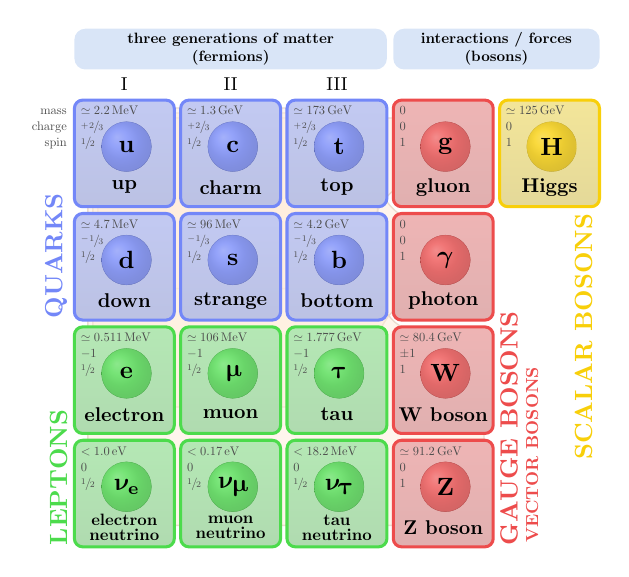
\begin{tikzpicture}[fillbox=1,x={(1.5,0)},y={(0,1.6)},global scale=0.9]
      
      % QUARKS
      \begin{scope}[alt={<4,10,14>{pic opacity=\d,opacity=\d}{}}] % to highlight others
        \pic[alt={{<7,8>{pic opacity=\d}{}}}] (QU) at (1,4) {
          particle={quarkcol}{u}{up}{%
            \simeq2.2\MeV}{\!\sfrac{+\!2}{3}}{\sfrac{1}{2}}
        };
        \pic[alt={<6,8>{pic opacity=\d}{}}] (QC) at (2,4) {
          particle={quarkcol}{c}{charm}{%
            \simeq1.3\GeV}{\!\sfrac{+\!2}{3}}{\sfrac{1}{2}}
        };
        \pic[alt={<6,7>{pic opacity=\d}{}}] (QT) at (3,4) {
          particle={quarkcol}{t}{top}{%
            \simeq173\GeV}{\!\sfrac{+\!2}{3}}{\sfrac{1}{2}}
        };
        \pic[alt={<7,8>{pic opacity=\d}{}}] (QD) at (1,3) {
          particle={quarkcol}{d}{down}{%
            \simeq4.7\MeV}{\!\sfrac{-\!1}{3}}{\sfrac{1}{2}}
        };
        \pic[alt={<6,8>{pic opacity=\d}{}}] (QS) at (2,3) {
          particle={quarkcol}{s}{strange}{%
            \simeq96\MeV}{\!\sfrac{-\!1}{3}}{\sfrac{1}{2}}
        };
        \pic[alt={<6,7>{pic opacity=\d}{}}] (QB) at (3,3) {
          particle={quarkcol}{b}{bottom}{%
            \simeq4.2\GeV}{\!\sfrac{-\!1}{3}}{\sfrac{1}{2}}
        };
        \node[below left,proplabel]
          at (0.5,4+0.5*\pw) {\strut mass};
        \node[below left,proplabel]
          at (0.5,4+0.35*\pw) {\strut charge};
        \node[below left,proplabel]
          at (0.5,4+0.20*\pw) {\strut spin};
        \node[quarkcol,bflabel,above right=0pt and -2pt]
          at (QD-sw) {QUARKS};
      \end{scope}
      
      % LEPTONS
      \begin{scope}[alt={<3,10,12,14>{pic opacity=\d,opacity=\d}{}}] % to highlight others
        \pic[alt={<7,8>{pic opacity=\d}{}}] (EL) at (1,2) {
          particle={leptoncol}{e}{electron}{%
            \simeq0.511\MeV}{-1}{\sfrac{1}{2}}
        };
        \pic[alt={<6,8>{pic opacity=\d}{}}] (MU) at (2,2) {
          particle={leptoncol}{$\unslant\mu$}{muon}{%
            \simeq106\MeV}{-1}{\sfrac{1}{2}}
        };
        \pic[alt={<6,7>{pic opacity=\d}{}}] (TAU) at (3,2) {
          particle={leptoncol}{$\unslant\tau$}{tau}{%
            \simeq1.777\GeV}{-1}{\sfrac{1}{2}}
        };
        % NEUTRINOS
        \begin{scope}[alt={<11>{pic opacity=\d,opacity=\d}{}}] % to highlight others
          \pic[alt={<7,8>{pic opacity=\d}{}},textscale=0.66] (NE) at (1,1) {
            particle={leptoncol}{$\PGn{\text{e}}$}{electron\\[-3pt]neutrino}{%
              <1.0\eV}{0}{\sfrac{1}{2}}
          };
          \pic[alt={<6,8>{pic opacity=\d}{}},textscale=0.66] (NM) at (2,1) {
            particle={leptoncol}{$\PGn{\unslant\mu}$}{muon\\[-3pt]neutrino}{%
              <0.17\eV}{0}{\sfrac{1}{2}}
          };
          \pic[alt={<6,7>{pic opacity=\d}{}},textscale=0.66] (NT) at (3,1) {
            particle={leptoncol}{$\PGn{\unslant\tau}$}{tau\\[-3pt]neutrino}{%
              <18.2\MeV}{0}{\sfrac{1}{2}}
          };
        \end{scope}
        \node[leptoncol,bflabel,above right=0pt and -2pt]
          at (NE-sw) {LEPTONS};
      \end{scope}
      
      % GAUGE BOSONS
      \begin{scope}[alt={<2-9,14>{pic opacity=\d,opacity=\d}{}}] % to highlight others
        \pic[alt={<11,13,15>{pic opacity=\d}{}}] (GLU) at (4,4) {
          particle={gaugecol}{g}{gluon}{%
            0}{0}{1}
        };
        \pic[alt={<12-13,15>{pic opacity=\d}{}}] (GAM) at (4,3) {
          particle={gaugecol}{$\gamma$}{photon}{%
            0}{0}{1}
        };
        \pic[alt={<11,12>{pic opacity=\d}{}}] (W) at (4,2) {
          particle={gaugecol}{$\mathrm{W}$}{W boson}{% %^\pm
            \simeq80.4\GeV}{\pm1}{1}
        };
        \pic[alt={<11,12>{pic opacity=\d}{}}] (Z) at (4,1) {
          particle={gaugecol}{$\mathrm{Z}$}{Z boson}{% %^0$
            \simeq91.2\GeV}{0}{1}
        };
        %%%\pic[pic opacity=\opWeak,textscale=0.7] (L) at (5.6,1) {
        %%%  particle={gaugecol}{LQ}{leptoquark}{% %^0$
        %%%    ?}{?}{1} %>1\TeV
        %%%};
        \node[gaugecol,bflabel,below right=0pt and 2pt]
          (GB) at (Z-se) {GAUGE BOSONS};
        \node[gaugecol,bflabel,below right=-1pt and 2pt,scale=0.7]
          at (GB.south west) {VECTOR BOSONS};
      \end{scope}
      
      % SCALAR BOSONS
      \begin{scope}[alt={<2-13>{opacity=\d,pic opacity=\d}{}}] % to highlight others
        \pic (HIG) at (5,4) {
          particle={scalarcol}{H}{Higgs}{%
            \simeq125\GeV}{0}{1}
        };
        \node[scalarcol,bflabel,above left=-2pt and 2pt]
          at (HIG-se) {SCALAR BOSONS};
      \end{scope}
      
      %%%% TENSOR BOSONS
      %%%\begin{scope}[alt=<2>{opacity=\d,pic opacity=\d}{opacity=1,pic opacity=1}] % to highlight others
      %%%  \pic (GRA) at (6,4) {
      %%%    particle={tensorcol}{G}{Graviton}{%
      %%%      0}{0}{2}
      %%%  };
      %%%  \node[tensorcol,bflabel,above left=-2pt and 2pt]
      %%%    (TB) at (GRA-se) {TENSOR BOSONS};
      %%%  \node[tensorcol,bflabel,above left=-1pt and 2pt,scale=0.7]
      %%%    at (TB.north east) {HYPOTHETICAL};
      %%%\end{scope}
      
      % HEADER
      \fill[mylightblue,rounded corners=4pt]
        (1-\pw/2,4.74) rectangle (3+\pw/2,5.1)
        node[midway,header] {%
          three generations of matter\\[0pt]
          (fermions)};
      \fill[mylightblue,rounded corners=4pt]
        (4-\pw/2,4.74) rectangle (5+\pw/2,5.1)
        node[midway,header] {%
          interactions / forces\\[0pt]
          (bosons)};
      \node[above=0pt,scale=0.75] at (1,4.5) {I};
      \node[above=0pt,scale=0.75] at (2,4.5) {II};
      \node[above=0pt,scale=0.75] at (3,4.5) {III};
      
      % INTERACTION GROUPS
      \ifnum0=0
      \begin{pgfonlayer}{back} % draw on back
        
        % STRONG INTERACTIONS
        \def\R{11.5pt}
        \fill[intgroup,alt={<2-11,13-15>{opacity=0.5*\d}{opacity=0.5}}] %=blue!20!white]
          (QU-p)++(0,\R) -- ($(GLU-p)+(0,\R)$) arc(90:-90:\R)
          to[out=-180,in=90,looseness=1.2] ($(QB-p)+(\R,0)$) arc(0:-90:\R)
          -- ($(QD-p)+(0,-\R)$) arc(-90:-180:\R)
          -- ($(QU-p)+(-\R,0)$) arc(180:90:\R)
          -- cycle;
        
        % ELECTROMAGNETIC INTERACTIONS
        \def\R{13.5pt}
        \fill[intgroup,alt={<2-10,12,13-15>{opacity=0.5*\d}{opacity=0.5}}] %=green!20!white]
          (QU-p)++(0,\R) -- ($(QT-p)+(0,\R)$) arc(90:0:\R)
          to[out=-90,in=180,looseness=1.2] ($(GAM-p)+(0,\R)$) arc(90:-90:\R)
          to[out=-180,in=90,looseness=1.2] ($(TAU-p)+(\R,0)$) arc(0:-90:\R)
          -- ($(EL-p)+(0,-\R)$) arc(-90:-180:\R)
          -- ($(QU-p)+(-\R,0)$) arc(180:90:\R)
          -- cycle;
        
        % WEAK INTERACTIONS
        \def\R{15.5pt}
        \fill[intgroup,alt={<2-12,14,15>{opacity=0.5*\d}{opacity=0.5}}] %=mypurple!20!white]
          (QU-p)++(0,\R) -- ($(QT-p)+(0,\R)$) arc(90:0:\R)
          -- ($(QB-p)+(\R,0)$)
          to[out=-90,in=180,looseness=1.4] ($(W-p)+(0,\R)$) arc(90:0:\R)
          -- ($(Z-p)+(\R,0)$) arc(0:-90:\R)
          -- ($(NE-p)+(0,-\R)$) arc(-90:-180:\R)
          -- ($(QU-p)+(-\R,0)$) arc(180:90:\R)
          -- cycle;
        
      \end{pgfonlayer}
      \fi
    
    \end{tikzpicture}
    
    % TEXT
    \column{0.48\linewidth}
    \begin{itemize}
      % FERMIONS
      \item<2-> \textbf{Fermions} of spin $1/2$, which make up matter
      \begin{itemize}
        \item<3-> {\color{quarkcol!80!black}\textbf{Quarks}}
        \item<4-> {\color{leptoncol!80!black}\textbf{Leptons}}
        \item<5-> Three generations
      \end{itemize}
      % GAUGE BOSONS
      \item<10-> {\color{gaugecol!80!black}\textbf{Gauge bosons}} of spin $1$, which mediate the fundamental interactions
      \begin{itemize}
        \item<11-> Electromagnetic interaction
        \item<12-> Strong interaction
        \item<13-> Weak interaction
      \end{itemize}
      \item<14-> One {\color{scalarcol!90!black}\textbf{scalar boson}} of spin $0$, which gives mass to fermions and weak bosons
    \end{itemize}
    \only<16>{}
  \end{columns}
\end{frame}

\end{document}